\part{Design, Proof, Implementation, and Synthesis of Hierarchical Cache-Coherence Protocols}

\chapter{Case Studies: Hierarchical MSI and MESI Protocols}
\label{sec-case-study}

In this chapter we specify, implement, and formally prove the correctness of the following three hierarchical cache-coherence protocols: an inclusive MSI protocol, a noninclusive MSI protocol, and a noninclusive MESI protocol.
Each protocol is parameterized by a tree $t$ that decides the topology of the memory subsystem $S$, thus the system naturally satisfies $\ontree{S}{t}$.
Cache objects in each protocol are defined using the rule templates (defined in \autoref{sec-rule-templates}) thus the system satisfies $\goodrules{S}{t}$ by construction.
These predicates imply that each protocol satisfies the serializability property, proven in \autoref{thm-sz-guarantee}.
We will see how \hemiola{} helps implement and prove the protocols by taking full advantage of serializability.

\section{Design Principles}
\label{sec-design-principles}

We first present the common design principles shared by all the case studies.

\subsection{Topology as a parameter}
\label{sec-topo-param}
Each design is parameterized by a tree $t$ that decides the topology of the memory subsystem.
In other words, whenever we instantiate the tree parameter, we get a cache-coherence design and its correctness proof for free.
For example, the following tree definition will generate a cache-coherence protocol for four L1 caches, two L2 caches, the last-level cache (LLC), and the main memory:
\begin{lstlisting}[numbers=none, frame=none]
Definition t: tree := Node [Node [Node [Leaf; Leaf]; Node [Leaf; Leaf]]].
\end{lstlisting}

There are three different kinds of caches in this topology-parameterized protocol.
First of all, there are L1 caches (denoted as $L_1$) that correspond to leaf nodes in the tree.
Symmetrically, each uses the same set of rules.
The second kind is the last-level cache (LLC), which is the only one attached to the main memory, the root of the tree.
It is possible to design multiple LLCs attached to the main memory in \hemiola{}, but our case studies follow standard practice in sticking to a single LLC.
All the other caches between the L1 caches and the LLC are called intermediate caches (denoted as $L_i$), and they share a common set of rules as well.

\subsection{Design and proof per-line}
\label{sec-design-line}

The protocol is defined just for a single cache line first and naturally extended to all cache lines using a protocol compiler that will be introduced in \autoref{sec-compiler}.
This approach is reasonable in terms of correctness, since a transaction does not affect coherence for lines other than its own.
Consider the ``duplicated'' protocol first, where each cache line, its status, a directory entry, communication channels, and a lock holder are all duplicated per-line.
It is infeasible to extend the protocol literally in this way, since we cannot require physically distinct channels and lock holders for all cache lines.
The protocol compiler restricts the resources (\eg{} channels, lock holders, etc.) to make the implementation hardware-synthesizable.
Note that in this sense the duplicated protocol can be regarded as the most general multiline design, whose behaviors can cover all the behaviors of compiled implementations (see \autoref{sec-compiler-correctness} for details).

\subsection{Nondeterministic invalidation/eviction}
\label{sec-nondet-inv-ev}

The protocol initiates invalidations and evictions nondeterministically.
In other words, there are rules in each cache that can be executed even without being triggered by input messages, to make invalidation requests to the child caches or to make an eviction request to the parent.
This design choice is certainly not realistic, but it always has more behaviors than any design with specific invalidation/eviction policy, thus in terms of correctness a refinement to the specific design is trivial.

For instance, a number of practical cache-coherence protocols manage a data structure (a cache) to keep track of least-recently-used (LRU) cache line per set (lines with the same index)~\cite{cacheLRU}.
Use of such a data structure and the decision algorithm is irrelevant to the correctness of a protocol.
In other words, a protocol with the LRU replacement policy, regardless of its implementation, always has less behaviors than the one with nondeterministic eviction.

Another instance is a back-invalidation policy used in an inclusive cache.
Back invalidation is necessary to maintain the cache inclusion among the parent and child caches and may happen right before evicting a parent cache line.
There is another practical policy, called self-invalidation~\cite{Ros:2012}, where some voluntary back invalidations happen to increase performance.
Similar to the case of cache replacement, a protocol with nondeterministic invalidation includes all the behaviors by the one with a specific invalidation policy.

\subsection{Directory-based coherence}
\label{sec-dir-based}

The protocol uses a directory structure to ensure coherence, introduced in \autoref{sec-design-space}.
In our designs, each node with children has its own directory structure to track their statuses.
The directory holds sound information about the status of each child \emph{subtree}.
For example, for a certain cache line, if an L1 cache $L_1$ has M status for the line, then all the ancestors (including the main memory) of $L_1$ have the directory status M pointing to the child subtree that contains $L_1$.

\subsection{Noninclusive-cache inclusive-directory (NCID) structure}
\label{sec-inc-noninc}

Our noninclusive protocols employ the noninclusive-cache inclusive-directory (NCID)~\cite{Zhao:2010} structure to optimize the cache space.
As explained in \autoref{sec-design-space}, in noninclusive protocols the parent cache does not have to contain all the line values that children have, and back invalidations are not required to evict a line.

Measuring performance among various cache-inclusion policies is beyond the scope of this thesis.
That said, we choose noninclusive caches as part of our case studies to demonstrate that \hemiola{} is general enough to design and prove various cache-coherence protocols, where specifically the noninclusive caches are the ones that most previous work had difficulty dealing with properly.

\section{The MSI Protocol}
\label{sec-msi-protocol}

The MSI protocol is known as a base cache-coherence protocol that can be optimized to more sophisticated protocols like MESI, MOSI, etc.
Even though it is a base protocol, there are a lot of nontrivial cases that require deep understanding of the protocol itself and the nature of distributed protocols, especially in hierarchical protocols.
In this section we design two hierarchical, directory-based MSI protocols, one with the inclusive cache-inclusion policy and the other with the noninclusive policy.
As explained in \autoref{sec-design-principles}, the description and the correctness proof are for a single cache line, parameterized by a tree deciding the system topology.

\subsection{Protocol description}
\label{sec-msi-protocol-desc}

\subsubsection{Cache states}

A cache state has the form $O(\textsf{st}, \textsf{v}, \textsf{dir}, \textsf{owned})$, consisting of a status, a value, a directory, and a Boolean called an \emph{ownership bit}.

A status is either \stM{}($=3$), \stS{}($=2$), \stI{}($=1$), or the ``Not Present'' status (\stNP{}$=0$), encoded by natural numbers.
\stNP{} means that the line does not exist in the cache object.
In our case-study protocols we distinguish \stI{} and \stNP{} to avoid unnecessary line creation when invalidating the line~\cite{ccbook:2020}.
That is, when the cache object gets an invalidation request, if the line status is \stNP{}, then it should not change its status to \stI{} but maintain the \stNP{} status.

A directory contains a status of its children called a \emph{directory status} and a list of child-cache indices that have the directory status.
We will denote the directory like $\dir{\stS{}}{1, 2}$, saying that the directory status is \stS{} and child subtrees with indices $1$ and $2$ may contain caches with \stS{} status.

The ownership bit is to determine whether the cache is responsible for writing the value back to the parent when invalidated.
When a cache has the \stM{} status, the ownership bit is always true.
However, when the cache has \stS{}, the ownership bit can be either true or false.
Note that $L_1$ does not have a directory since it has no children.
It also does not have an ownership bit, since it does not have a case where it has \stS{} status but is responsible for writing the value back.

\tikzset{
  pcc1/.pic = {
    \node at (0, 0) {$P(\stI{}, \cdot, \dir{\stM{}}{1}, \bot)$};
    \node at (-1.5, -1.5) {$C_1(\stM{}, v)$};
    \node at (1.5, -1.5) {$C_2(\stI{}, \cdot)$};
    % to the parent of P
    \node at (0, 1.2) {$\vdots$};
    \draw [>->] (-0.2, 0.4) -- (-0.2, 0.8);
    \draw [>->] (0, 0.4) -- (0, 0.8);
    \draw [<-<] (0.2, 0.4) -- (0.2, 0.8);
    % between P and C_1
    \draw [<-<] (-0.7, -0.4) -- (-1.3, -1.1);
    \draw [<-<] (-0.5, -0.4) -- (-1.1, -1.1);
    \draw [>->] (-0.3, -0.4) -- (-0.9, -1.1);
    % between P and C_2
    \draw [>->] (0.7, -0.4) -- (1.3, -1.1);
    \draw [<-<] (0.5, -0.4) -- (1.1, -1.1);
    \draw [<-<] (0.3, -0.4) -- (0.9, -1.1);
    % message
    \node[color=myblue,label={[label distance=-10pt]below left:{\blmsgsm{rqS}}}] at (0.6, -0.75) {$\bullet$};
  },
  pcc2/.pic = {
    \node at (0, 0) {\color{myred} $P(\stS{}, v, \dir{\stS{}}{1,2}, \top)$};
    \node at (-1.5, -1.5) {\color{myred} $C_1(\stS{}, v)$};
    \node at (1.5, -1.5) {$C_2(\stI{}, \cdot)$};
    % to the parent of P
    \node at (0, 1.2) {$\vdots$};
    \draw [>->] (-0.2, 0.4) -- (-0.2, 0.8);
    \draw [>->] (0, 0.4) -- (0, 0.8);
    \draw [<-<] (0.2, 0.4) -- (0.2, 0.8);
    % between P and C_1
    \draw [<-<] (-0.7, -0.4) -- (-1.3, -1.1);
    \draw [<-<] (-0.5, -0.4) -- (-1.1, -1.1);
    \draw [>->] (-0.3, -0.4) -- (-0.9, -1.1);
    % between P and C_2
    \draw [>->] (0.7, -0.4) -- (1.3, -1.1);
    \draw [<-<] (0.5, -0.4) -- (1.1, -1.1);
    \draw [<-<] (0.3, -0.4) -- (0.9, -1.1);
    % message
    \node[color=myred,label={[label distance=-14pt]above right:{\rdmsgsm{rsS}{\color{myred}$(v)$}}}] at (1.0, -0.75) {$\bullet$};
  }
}
\begin{figure}[h]
  \centering
  \begin{tikzpicture}
    \pic at (-3.2, 0) {pcc1};
    \node at (0, 0) {$\Longrightarrow$};
    \pic at (3.2, 0) {pcc2};
  \end{tikzpicture}
  \caption{An ownership bit set in a shared-state cache}
  \label{fig-ownership-bit}
\end{figure}

\autoref{fig-ownership-bit} presents an example of a shared-state cache having its ownership bit set in a hierarchical memory subsystem.
It could happen when an L1 cache $C_2$ wants to get \stS{} while another L1 cache $C_1$ has \stM{}.
In this case, $C_2$ sends \blmsg{rqS} and waits for the response with the value \rdmsg{rsS}{\color{myred}$(v)$}.
After a few steps, the value is pulled from $C_1$, and the parent $P$ gets the data as well, entering a shared status with ownership bit set.
Here the bit says that the shared value might be dirty, so it should be written back.

The ownership bit intuitively constrains which caches can have valid status.
In the figure, all the other caches outside $P$, after pulling a value from $C_1$, are in the invalid status, since previously $C_1$ had the dirty value with \stM{}.
We will see how this intuition is used for the correctness proof soon in \autoref{sec-msi-proof}.

\subsubsection{Protocol description with rule templates}

We present a number of rule descriptions in the MSI protocols that employ the rule templates provided in \hemiola{}.
Each rule template is defined in Coq, taking in several parameters and generating a rule.
We exploited Coq's notation mechanism to have a compact definition for each rule template.

\begin{figure}[h]
  \centering
\begin{lstlisting}[escapeinside={(*}{*)}]
Definition l1GetSRqUpUp: Rule :=
  rule.rquu
  :accepts getRq
  :from cidx
  :me oidx
  :requires (fun ost msgIn => ost#[status] (*$\leq$*) msiI)
  :transition (fun ost msgIn => <| rqS; 0 |>).
\end{lstlisting}
  \caption{$L_1$ requesting \stS{} to the parent}
  \label{fig-rule-l1-rqS}
\end{figure}

\autoref{fig-rule-l1-rqS} presents an actual rule definition, starting with an invocation of a particular rule template \slstinline{rule.rquu}, which takes a request from one of its children and sends a further request to the parent.
An L1 cache does not have any children; in this case \slstinline{cidx} will be instantiated to an abstract node referring to the external interface (\ie{} processor core) for it.
Each line starting with a colon (\slstinline{:}) provides more information about the rule.
This rule \slstinline{accepts} a message with the ID \slstinline{rqS} \slstinline{from} the child with the index \slstinline{cidx}.
This rule template also requires to write down which object (cache) it belongs to (\slstinline{me}), the precondition (\slstinline{requires}), and the state-transition function (\slstinline{transition}).
The output \slstinline{rqS} message that we generate carries no data value, so we pair it with a dummy zero value.

Each rule template has different (Coq) types for a precondition and a state-transition function.
In this example rule, the precondition takes the current object state (\slstinline{ost}) and an input message (\slstinline{msgIn}) from the child.
It suffices to say that the current status is either \stI{} or \stNP{} (\slstinline{ost#[status]} $\leq$ \slstinline{msiI}), thus the cache needs to request to the parent.
Note that the statuses are defined as natural numbers, so we can use arithmetic operations inside the precondition.

The transition function also takes the current object state and the input message, and it returns only the message to the parent.
In this example the cache forwards \slstinline{rqS} to the parent without any meaningful value.
As explained in \autoref{sec-rule-templates}, when forwarding a request to the parent, no state transition should happen except locking.
The rule template ensures this requirement by restricting the type of the transition function.
Note that the rule does not mention locking at all.
Each rule template automatically sets a proper lock; in this case an uplock is set right after sending a request to the parent.

\begin{figure}[h]
  \centering
\begin{lstlisting}
Definition liDownSRsUpDownM: Rule :=
  rule.rsudo
  :accepts downRsS
  :holding rqS
  :requires (fun _ _ _ => True)
  :transition (fun ost rsFrom rs rq rsbTo =>
    (ost +#[status <- msiS]
         +#[val <- rs.(msg_value)]
         +#[dir <- setDirS [rsbTo; rsFrom]]
         +#[owned <- true],
     <| rsS; rs.(msg_value) |>)).
\end{lstlisting}
  \caption{$L_i$ responding to the child that requested \slstinline{rqS}}
  \label{fig-rule-li-downRsS}
\end{figure}

\autoref{fig-rule-li-downRsS} presents another example rule that is fired at the last of the steps shown in \autoref{fig-ownership-bit}, which sends the response to the child who requested \slstinline{rqS}.
Template \slstinline{rule.rsudo} says that the rule takes a single response and responds back to the original requestor.
The rule \slstinline{accepts} the response message with the ID \slstinline{downRsS}.
This rule can be executed when it is \slstinline{holding} a downlock, where the holder contains the original request message with the ID \slstinline{rqS}.
While the rule does not require any additional precondition (\slstinline{fun _ _ _ => True}), it changes the object state, unlike rules that make requests.

The transition function takes the current object state (\slstinline{ost}), the object index that sent a response (\slstinline{rsFrom}), the response message (\slstinline{rs}), the original request in a lock holder (\slstinline{rq}), and the index of the original requestor (\slstinline{rsbTo}).
The transition returns a pair of the next state and an output message; this rule sets its status to \stS{}, stores the up-to-date value brought from the \slstinline{downRsS} message, sets the directory status to \stS{} by adding the two children -- one that was downgraded to \stS{} before and the other that originally requested \stS{} -- as sharers, and sets the ownership bit as true since the up-to-date value might be dirty in this case.
It also sends a response (\slstinline{rsS}) to the requestor with the up-to-date value. Lastly, the rule automatically releases the downlock.

\begin{figure}[h]
  \centering
\begin{lstlisting}[escapeinside={(*}{*)}]
Definition liDropImm: Rule :=
  rule.imm
  :requires (fun ost _ _ => ost#[status] <= msiS (*$\wedge$*) ost#[owned] = false)
  :transition (fun ost => ost +#[status <- msiNP]).
\end{lstlisting}
  \caption{$L_i$ immediately dropping a line}
  \label{fig-rule-li-drop-imm}
\end{figure}

\autoref{fig-rule-li-drop-imm} is a rule only used in the noninclusive protocol.
Template \slstinline{rule.imm} is for making an immediate state transition that neither takes any input messages nor generates any output messages.
Its precondition just says that the line is possibly shared but needs not be written back (the ownership bit is false).
In this case, we can \emph{silently} drop the line by setting the status to \stNP{}, to denote explicitly that the line is removed.
Note that there is no precondition about the directory status at all; a line can be dropped even when the directory status is \stS{} or \stM{}, which is not allowed in inclusive caches.
Our noninclusive protocol employs NCID, and in this case the dropped line may migrate to so-called the extended directory~\cite{Zhao:2010}.
We will see in \autoref{sec-compiler} how this migration is implicitly processed in the actual hardware implementation.

\begin{figure}[h]
  \centering
\begin{lstlisting}
Definition liBInvRqS: Rule :=
  rule.rqsd
  :requires (fun ost => ost#[dir].(dir_st) = msiS)
  :transition (fun ost => (ost#[dir].(dir_sharers), <| downRqIS; O |>)).

Definition liBInvRqM: Rule :=
  rule.rqsd
  :requires (fun ost => ost#[dir].(dir_st) = msiM)
  :transition (fun ost => ([ost#[dir].(dir_excl)], <| downRqIM; O |>)).
\end{lstlisting}
  \caption{$L_i$ initiating a back invalidation}
  \label{fig-rule-li-back-inv}
\end{figure}

Lastly, \autoref{fig-rule-li-back-inv} shows two rules to initiate back invalidation, only used in the inclusive protocol.
Template \slstinline{rule.rqsd} is for making downward requests without any input messages.
\slstinline{liBInvRqS} \slstinline{requires} the directory status to be \stS{}, and in this case it makes downward requests to the sharers.
On the other hand, \slstinline{liBInvRqM} \slstinline{requires} the directory status to be \stM{}, and in this case it makes a single downward request to the exclusive child cache.

It is worth recalling that thanks to the rule templates, rule descriptions in the protocol never mention anything about how to set/release locks to deal with interleavings safely; they are rather designed as if only a single transaction is being processed when executing a rule.

\subsection{Correctness proof}
\label{sec-msi-proof}

Now we present the correctness proof of the MSI protocol, claiming that the implementation refines to a single-line memory as a spec.
We already discussed in \autoref{sec-pred-msg} that a number of invariants are necessarily required to prove simulation.
The two variants -- inclusive and noninclusive protocols -- have different set of rules but require the same invariants.
In this section, we provide necessary invariants to prove the correctness of the MSI protocol, and we demonstrate how \hemiola{} helps prove such invariants using predicate messages.

\subsubsection{Logical status of a cache}
Before talking about invariants, we would like to clarify how to deal with cache statuses in transition.
For example, what would be the representative cache status if a cache currently has a status \stS{} but is just about to handle the eviction response (say \msgsfsm{rsPut}) that will remove the line?
It implies that the parent directory already accepted the eviction request and changed the directory status (for the child) properly.
In this case, it would make more sense to regard the child cache status to \stI{}.

In order to deal with this situation, we introduce a notion called \emph{logical status} to obtain an abstract status of each cache.
In the above example, even if the cache has not handled \msgsfsm{rsPut} yet, the logical status is \stI{}.
Logical statuses are defined formally as follows:
\begin{itemize}
\item A cache has logical status \stM{} iff it has \stM{} and there is no \msgsfsm{rsPut} to it.
\item A cache has logical status \stS{} iff either 1) it has \stS{} and there is no \msgsfsm{rsPut} to it or 2) there is a response \msgsfsm{rsS} to it.
\item A cache has logical status \stI{} iff either 1) it has \stI{} and there is no \msgsfsm{rsM} or \msgsfsm{rsS} to it or 2) there is a response \msgsfsm{rsPut} to it.
\end{itemize}
Note that the logical status of a cache is \emph{not} \stM{} when there is a response \msgsfsm{rsM} to it, since the response could still imply an ongoing invalidation process.
We will see the actual use case of the \msgsfsm{rsM} message very soon in \autoref{fig-pred-msg-msi}.

\paragraph{Invariants.}
The MSI protocol largely requires three invariants, where each invariant corresponds to a desired property of one status -- \stM{}, \stS{}, and \stI{}.

\begin{invariant}[Exclusiveness invariant]
  \label{inv-excl}
  Whenever a cache object $O$ has logical status \stM{}, then all the other caches are in logical \stI{} status.
  We denote this predicate by $\objsinv{\lambda c.\; c \neq O}$, where $\objsinv{S}$ claims that any cache object in the object set $S$ has logical \stI{} status.
\end{invariant}

\begin{invariant}[Sharing invariant]
  \label{inv-sharing}
  All caches in logical \stS{} status have the same coherent value.
\end{invariant}

\begin{invariant}[Invalidness invariant on ownership bits]
  \label{inv-inv-ownership}
  If a cache $C$ has an ownership bit true, then all the caches outside $C$ (\ie{} \subtreec{C}) have logical \stI{} status, \ie{} $\objsinv{\subtreec{C}}$.
\end{invariant}

\begin{invariant}[Invalidness invariant on directory status \stM{}]
  \label{inv-inv-dir-m}
  If a parent $P$ has a directory status $M$ to a child $C_i$, then all the caches outside $C_i$ (including $P$) have logical \stI{} status, \ie{} $\objsinv{\subtreec{C_i}}$.
\end{invariant}

The sharing invariant (\autoref{inv-sharing}) is the easiest one to prove, since the rules involved with sharing the coherent value employ just simple value forwarding.
For example, the rule in \autoref{fig-rule-li-downRsS} just takes a message \slstinline{downRsS} that contains the coherent value and stores/sends the value.
Proving the preservation of the invariant for this rule is very straightforward.

\subsubsection{Invariant proofs using predicate messages}

While proving the sharing invariant is easy, it is nontrivial to prove the exclusiveness (\autoref{inv-excl}) and invalidness invariants (\autoref{inv-inv-ownership} and \autoref{inv-inv-dir-m}), since these invariants are involved with global cache states.
We have already learned in \autoref{sec-pred-msg} that in order to prove this kind of invariants, it is desirable to state some supporting invariants based on the existence of certain messages, called predicate messages.
We also discovered that on top of serializability it is much easier to state and prove predicate messages.

\begin{figure}[t]
  \centering
  \begin{tikzpicture}
    %% Part 1
    \node [color=myblue] at (0, 1.2) {$(P.\textsf{owned} = \top)\{\objsinv{\subtreec{P}}\}$};
    \node at (0, 0) {$P$};
    \node at (-1.2, -1.2) {$C_0$};
    \node at (0, -1.5) {$C_1$};
    \node at (1.3, -0.9) {$C_n$};

    \draw [dotted,line width=1pt] (0, 0.4) -- (0, 0.8);
    \draw [>->] (-0.3, -0.3) -- (-0.9, -0.9);
    \draw [>->] (0, -1.2) -- (0, -0.3);
    \draw [>->] (1.0, -0.7) -- (0.3, -0.2);
    \draw [loosely dotted,line width=1pt] (0.4, -1.5) to[out=0,in=-150] (1.1, -1.1);

    \node [color=myblue,label={[myblue,label distance=-9pt]below right:{\msgsfsm{rsI}}}] at (0, -0.7) {$\bullet$};
    \node [color=myblue,label={[myblue,label distance=-9pt]above right:{\predmsg{\msgsfsm{rsI}}{\objsinv{\subtree{C_n}}}}}] at (0.65, -0.45) {$\bullet$};
    \node [color=myred,label={[myred,label distance=-9pt]above left:{\predmsg{\msgsfsm{rsM}}{\objsinv{\subtreec{C_0}}}}}] at (-0.6, -0.6) {$\bullet$};

    \node [anchor=west,draw] at (1.8, -1.4) {{\small {\color{myblue} current}/{\color{myred} next}}};

    %% Part 2
    \node [color=mygray] at (-2.4, -2.4) {$L_1$};
    \node [color=mygray,anchor=west] at (-1.8, -2.7) {$(L_1.\textsf{st} = M)\{\objsinv{\lambda c. c \neq L_1}\}$};
    \draw [color=mygray,dotted,line width=1pt] (-1.7, -2.7) -- (-2.1, -2.4);
    \draw [loosely dotted,line width=1pt] (-1.4, -1.4) -- (-1.7, -1.7);
    \draw [color=mygray,>->] (-1.8, -1.8) -- (-2.2, -2.2);

    \node [anchor=east,draw] at (-3.0, -2.4) {{\small\color{mygray} eventually}};

    \node [color=mygray,label={[label distance=-9pt,mygray]above left:{\predmsg{\msgsfsm{rsM}}{\objsinv{\subtreec{L_1}}}}}] at (-2.0, -2.0) {$\bullet$};
  \end{tikzpicture}
  \caption{Use of predicate messages to prove the exclusiveness invariant}
  \label{fig-pred-msg-msi}
\end{figure}

We would like to present a practical usage of predicate messages in proving the exclusiveness invariant, shown in \autoref{fig-pred-msg-msi}.
Suppose that an L1 cache (shown as {\color{mygray} $L_1$ in gray} in the figure) requested to the parent to get the \stM{} status.
When it finally handles the response \msgsfsm{rsM}, it should know all the other caches (except itself) have the logical \stI{} status to prove the exclusiveness invariant (denoted as {\color{mygray} $\{\objsinv{\lambda c. c \neq L_1}\}$}).
This proof case can be supported using the predicate message for \msgsfsm{rsM}, stating \objsinv{\subtreec{C}} (outside of the subtree rooted to $C$) when the message goes to $C$.
Since $L_1$ is the leaf node in the tree, it is trivial to prove $(\objsinv{\subtreec{L_1}} \to \objsinv{\lambda c. c \neq L_1})$, so we see an example of a predicate message helping prove a conventional invariant.

\autoref{fig-pred-msg-msi} also shows another case, where conventional invariants and predicate messages coordinate to prove a predicate message for the next state.
When a child $C_i$ sends the invalidation response \msgsfsm{rsI}, it should know that all the caches inside the subtree of $C_i$ have been invalidated (denoted as {\color{myblue} \objsinv{\subtree{C_i}}}).
When the parent $P$ subsequently handles the invalidation responses, it responds with \msgsfsm{rsM} to the original requestor ($C_0$ in the figure), requiring to prove {\color{myred} \objsinv{\subtreec{C_0}}}.
While $P$ also changes its status to \stI{} in this state transition, how do we infer that the caches outside $P$ are in the logical \stI{} status, which is required to prove the predicate over {\color{myred} \msgsfsm{rsM}}?
In this case, we should prove a simple object-level invariant of $P$ that it has the ownership bit true.
Then we can use \autoref{inv-inv-ownership} to obtain the desired predicate (denoted as {\color{myblue} $(P.\textsf{owned} = \top)\{\objsinv{\subtreec{P}}\}$}).
Combining all the predicates and the state transition by $P$, we can prove the next predicate message for {\color{myred} \msgsfsm{rsM}}.

\subsubsection{Refinement proof}

Once equipped with sufficient invariants, it is straightforward to prove the refinement between the implementation and the spec.
The only work is to define a correct simulation that relates all the coherent values in the implementation and the single value in the spec.
The coherent values are collected by looking at the logical status of each object; if the logical status is \stS{} or \stM{} then values either in the object or in some messages (\eg{} \slstinline{rsS}) are coherent.

Denoting by $\implcoh{s}{o}{v}$ that an object $o$ contains a coherent value $v$ in a system state $s$, the simulation can be stated as follows:
\begin{theorem}[Correctness of the MSI protocol]
  \label{thm-msi-correct}
  The following simulation relation holds between the implementation system state $s^I$ and the spec system state $s^S$.
  \begin{displaymath}
    s^I \sim s^S \triangleq \exists v.\; \forall o.\; \implcoh{s^I}{o}{v} \wedge s^S = \speccoh{v}.
  \end{displaymath}
  where $\speccoh{v}$ represents a single-value state for the spec.
\end{theorem}

\section{The MESI Protocol}
\label{sec-mesi-protocol}

The MESI protocol~\cite{Papamarcos:1984} applies further optimizations to the MSI protocol, by adding a status called Exclusive-Unmodified.
As the name of the status says, if a cache line has \stE{} status, then the line is exclusive to the cache but also clean.
In this section we present a hierarchical MESI protocol and demonstrate that the design and the correctness proof are easily extended from the ones for the MSI protocol with the support of \hemiola{}.

\subsection{Protocol description}
\label{sec-mesi-protocol-desc}

\subsubsection{Cache states}

The cache state in the MESI protocol is the same as in the MSI protocol, taking the form $O(\textsf{st}, \textsf{v}, \textsf{dir}, \textsf{owned})$.
The only difference is that the status may be \stE{}.

\subsubsection{New rules added beyond the MSI protocol}

There are several rules added in order to deal with the \stE{} status.
Like the previous rule-template examples, proper preconditions and transitions are automatically set in terms of locking.

\begin{figure}[h]
  \centering
\begin{lstlisting}
Definition l1GetMImmE: Rule :=
  rule.immd
  :accepts rqM
  :from cidx
  :requires (fun ost _ _ => ost#[status] = mesiE)
  :transition
     (fun ost msg => (ost +#[status <- mesiM]
                          +#[val <- msg.(msg_value)],
                      <| rsM; 0 |>)).
\end{lstlisting}
  \caption{$L_1$ silently upgraded to \stM{}}
  \label{fig-rule-l1-silent-upgrade}
\end{figure}

\autoref{fig-rule-l1-silent-upgrade} shows a basic case, where an L1 cache is silently upgraded from \stE{} to \stM{} to write data.
Template \slstinline{rule.immd} says that it takes a request from the external world (similar to \autoref{fig-rule-l1-rqS}) and immediately sends an external response.
As defined in the state \slstinline{transition} function, the cache silently changes its status to \stM{}, stores the new value from the input message, and responds with \slstinline{rsM}.

\begin{figure}[h]
  \centering
\begin{lstlisting}[escapeinside={(*}{*)}]
Definition liGetSImmME: Rule :=
  rule.immd
  :accepts rqS
  :from cidx
  :requires (fun ost _ _ => mesiE (*$\leq$*) ost#[status] (*$\wedge$*)
                            ost#[dir].(dir_st) = mesiI)
  :transition (fun ost _ => (ost +#[status <- mesiI]
                                 +#[dir <- setDirE cidx],
                             <| rsE; ost#[val] |>)).
\end{lstlisting}
  \caption{$L_i$ responding with \slstinline{rsE}}
  \label{fig-rule-li-rsE}
\end{figure}

Another case, shown in \autoref{fig-rule-li-rsE}, happens when an intermediate cache gets a request from a child to read the data, while it has status \stE{} or \stM{}.
In this case, instead of responding with \slstinline{rsS}, the cache sends \slstinline{rsE} to provide \stE{}.
Once the original requestor obtains \stE{} status, it can both read and write the data.

\subsection{Correctness proof}
\label{sec-mesi-proof}

\subsubsection{Logical status and new invariants for \stE{}}

We extend the notion of logical status from the MSI protocol, declaring that a cache in MESI is \stE{} if either 1) it has \stE{} and there is no eviction response to it or 2) there is a response \slstinline{rsE} to it.
We should extend the invariants as well to cover caches with \stE{} status.
\begin{itemize}
\item The exclusiveness invariant (\autoref{inv-excl}) also applies to \stE{}; whenever a cache has logical status \stE{}, all the other caches are logically in \stI{}.
\item The sharing (\autoref{inv-sharing}) and invalidness invariants (\autoref{inv-inv-ownership} and \autoref{inv-inv-dir-m}) remain the same.
\item A new invariant for \stE{} claims that if a cache takes an eviction request \emph{without writeback} from a child, and the directory status pointing to the child is \stE{}, then it has a coherent value.
\end{itemize}

\subsubsection{Invariant and refinement proofs}

Unlike the exclusiveness and the invalidness invariants, the invariant for \stE{} does not involve a large chunk of caches; it is rather an invariant that just relates a child and the parent cache states.
Therefore, we do not employ predicate messages in this invariant proof, instead using a normal induction on state-transition steps.

The simulation relation for the MESI protocol is just the same as the one for the MSI protocol, while the coherence predicate $\implcoh{s^I}{o}{v}$ is extended slightly to cover caches with \stE{} status and messages with ID \slstinline{rsE}.

\chapter{Compilation and Synthesis to Hardware}
\label{sec-comp-syn}

As mentioned in \autoref{sec-design-line}, so far we have dealt with cache-coherence protocols for a single line, where the specification has a single line as well.
In order to build a hardware-synthesizable multiline implementation, we developed a simple compiler that takes a single-line \hemiola{} protocol as a source program and generates a multiline implementation described in Kami~\cite{kami}.
Kami is a hardware formal-verification framework, where its own HDL and proof tools are defined in Coq, allowing users to design, specify, verify, and synthesize their hardware components.

The protocol transition system and the rule templates given in the \hemiola{} DSL match well rule-based HDLs like Kami; a rule in \hemiola{} naturally maps to an equivalent rule in Kami, which describes atomic state transitions in hardware modules.
Instead of directly compiling \hemiola{} protocols to a register-transfer language (RTL), we chose to build a compiler from \hemiola{} to Kami as a first step toward using the protocols and their correctness proofs within larger Kami proofs including processors -- though this thesis does not include those composition proofs.
Since Kami already has a hardware-synthesis toolchain, we can just compile a \hemiola{} program to Kami and use the toolchain to run it on FPGAs.

In this chapter, we will explore how a single-line \hemiola{} protocol is compiled to a multiline cache-coherence protocol implementation in Kami and demonstrate its synthesis to hardware (FPGA).
We will further discuss the desired specification of the multiline implementations, which is naturally derived from the source \hemiola{} protocol.

\section{Compilation of a \hemiola{} Protocol}
\label{sec-compiler}

\subsection{Compiler ingredients}

\begin{figure}[t]
  \centering
  \tikzstyle{arg} = [inner sep=1pt, outer sep=2pt]
  \tikzstyle{component} = [rectangle, draw=black, inner sep=5pt, outer sep=2pt]
  \tikzstyle{libcomp} = [rectangle, draw=black, minimum width=3.0cm, inner sep=5pt, outer sep=1pt]
  \tikzstyle{arrow}=[-{stealth}]
  \tikzstyle{dataflow}=[-{latex}]
  \begin{tikzpicture}
    \node[arg] (hemiolaSource) at (0, 2.0) {\sf{(Single-line) \hemiola{} protocol}};
    \node[component] (compiler) at (0, 0) {\sf{Protocol Compiler}};
    \node[arg, fill=white] (kamiTarget) at (0, -2.0) {\sf{(Multiline) Kami implementation}};
    \node[anchor=east, arg] (extComp) at (-2.5, 0.4) {\small\sf{Custom data structure reifier/compiler}};
    \node[anchor=east, arg] (cacheConfig) at (-2.5, -0.4) {\small\sf{Cache/MSHR configuration}};

    \node[anchor=west,
      rectangle, draw=black,
      minimum width=3.6cm,
      minimum height=2.2cm] (lib) at (3.0, 0) {};
    \node[above right] at (lib.north west) {\small\sf{Prebuilt Kami library}};
    \node[anchor=west, libcomp] (caches) at (3.3, 0.7) {\small\tt{Caches}};
    \node[anchor=west, libcomp] (victimlines) at (3.3, 0) {\small\tt{Victim lines}};
    \node[anchor=west, libcomp] (mshrs) at (3.3, -0.7) {\small\tt{MSHRs}};

    \draw [dataflow] (hemiolaSource) to
    node[left, inner sep=1pt] (reifyArrow) {}
    node[right] {\footnotesize\sf\it{after reification}} (compiler);
    \draw [dataflow] (compiler) to (kamiTarget);
    \draw [arrow] (extComp) to[out=0,in=180] (reifyArrow);
    \draw [arrow] (extComp) to[out=0,in=180] (compiler);
    \draw [arrow] (cacheConfig) to[out=0,in=180] (compiler);
    \draw [arrow] (lib) to[out=180,in=0] (compiler);

    \node[arg] (bsvTarget) at (0, -3.4) {\sf{Bluespec implementation}};
    \node[arg] (fpga) at (0, -4.8) {\sf{Circuit on FPGA}};

    \draw [dataflow] (kamiTarget) to[out=270,in=90,outer sep=3pt] node[left] {\footnotesize\sf\it{Kami-to-Bluespec transliteration}} (bsvTarget);
    \draw [dataflow] (bsvTarget) to[out=270,in=90,outer sep=3pt] node[left] {\footnotesize\sf\it{Bluespec synthesis}} (fpga);

    \begin{pgfonlayer}{bg}
      \node[anchor=west, text=mygray, arg] at (-8.5, -1.6) {\small\sf\it{compilation}};
      \draw[dashed] (-8.5, -2.0) -- (6.5, -2.0);
      \node[anchor=west, text=mygray, arg] at (-8.5, -2.4) {\small\sf\it{synthesis}};
    \end{pgfonlayer}
  \end{tikzpicture}
  \caption{Compilation and Synthesis of \hemiola{} protocols}
  \label{fig-compiler}
\end{figure}

\autoref{fig-compiler} depicts a compilation/synthesis flow from a given \hemiola{} protocol to an FPGA-ready circuit.
We provide an overview for each ingredient in the compiler, following the diagram.

\subsubsection{Preprocessing: reification}

A source program of the protocol compiler is a single-line protocol described in \hemiola{} with the rule templates.
Before feeding a \hemiola{} source program to the compiler, a preprocessing step is required, which is to reify the program into an AST we can hand off to the compiler.
\hemiola{} supports automated, correct-by-construction reification driven by a series of tactics in Coq.
For instance, the rule-reification tactic (\slstinline{reify_rule}) reifies a \hemiola{} rule to the corresponding rule AST, where \slstinline{HRule} is a Coq record (struct) containing the AST and its correctness, \ie{} denotation of the AST matches the denotation of the original rule:
\begin{lstlisting}[numbers=none, frame=none]
    Definition hl1GetMImmE: HRule l1GetMImmE := ltac:(reify_rule).
\end{lstlisting}

\subsubsection{Kami: the target register-transfer-level language}

Kami~\cite{kami} is a hardware-verification framework embedded in Coq with its own HDL at the register-transfer level.
A hardware design in Kami consists of modules with encapsulated private state (registers), public methods, and \emph{rules} that make atomic state changes.
Rules are fired by a global scheduler by Bluespec, later synthesized to the corresponding scheduling circuitry.
The Bluespec scheduler tries to find a maximal number of rules to execute at a cycle, with the convenient semantic guarantee that the execution can be interpreted as if the rules are executed atomically and sequentially, called \emph{one-rule-at-a-time execution}.

As mentioned in \autoref{sec-cc-as-mp}, the underlying transition system of \hemiola{} is also rule-based, and the semantics is based on the one-rule-at-a-time execution.
In this sense, Kami is a good target HDL in that a rule in \hemiola{} can be compiled to a corresponding rule in Kami.

Another advantage of using Kami as a target language is its verification tools defined in Coq.
Similarly to \hemiola{}, Kami also employs trace refinement as a correctness criterion.
Kami as a formal-verification framework provides an effective verification technique called \emph{modular refinement}, which basically says that trace refinement proofs of submodules can be combined together to obtain the refinement for the whole module:
\begin{theorem}[Modular refinement in Kami]
  \label{thm-kami-modular-refinement}
  \begin{displaymath}
    \forall I_1, I_2, S_1, S_2.\; I_1 \sqsubseteq S_1 \wedge I_2 \sqsubseteq S_2 \to I_1 + I_2 \sqsubseteq S_1 + S_2.
  \end{displaymath}
\end{theorem}

A corollary of \autoref{thm-kami-modular-refinement} is called \emph{modular substitution}, where we can substitute a submodule to another submodule to have a simpler design as an intermediate step to the final refinement:
\begin{theorem}[Modular substitution in Kami]
  \label{thm-kami-modular-subst}
  \begin{displaymath}
    \forall I_1, I_2, I_1'.\; I_1 \sqsubseteq I_1' \to I_1 + I_2 \sqsubseteq I_1' + I_2.
  \end{displaymath}
\end{theorem}
This corollary will be referred to when substituting our optimized cache-controller submodules in the entire memory subsystem to simpler ones, explained in \autoref{sec-compiler-correctness}.

\subsubsection{Reification and compilation of custom data structures}

Since a \hemiola{} protocol may use its own custom data structure (\eg{} directory structure for the MESI protocol), the compiler requires a user to provide a reifier and a compiler for it.
This task is straightforward for the user, since both reification and compilation work at the level of expressions, not rules.
For instance, a field access \slstinline{dir.(dir_sharers)} for a Coq record \slstinline{dir} is reified to an expression AST node \slstinline{(HDirGetSh hdir)}, where \slstinline{hdir} is the reified directory structure, and compiled to \slstinline{cdir@."dir_sharers"} in Kami, which uses a field-access expression.

\subsubsection{Prebuilt cache-related components}

The compiler uses prebuilt hardware components described in Kami.
Some of them are for implementing NCID~\cite{Zhao:2010} introduced in \autoref{sec-inc-noninc}, whose interfaces include asynchronous read and write of the line information (ownership bits, statuses, directory statuses, etc.) and value.
The cache normally uses a primitive BRAM (block RAM) module in Kami, later synthesized to a BRAM on an FPGA.
The cache module also manages \emph{victim lines} that should be evicted eventually.

Another prebuilt component holds a finite number of MSHRs, whose abstract interface includes registering, updating, and releasing MSHRs with respect to their types (uplock or downlock) and locking addresses.
Recall that ideally (as a spec) MSHRs are assigned per-line, but the actual design can contain only a finite number of them.
The compiler takes several counts as configuration parameters to determine the sizes of caches (\eg{} the number of lines and ways) and MSHRs (\eg{} the number of uplocks and downlocks).

\subsection{Compilation of a pipelined cache module}

One of the biggest differences between a source \hemiola{} protocol and the target Kami code is that the target accesses multiple lines \emph{asynchronously}.
In the source protocol, a single line can be read (or written) \emph{immediately} by directly accessing a value, whereas in the target the value is accessed asynchronously by making a read (or write) request with a certain line address to a cache and by handling the response.

\begin{figure}[t]
  \centering
  \renewcommand{\arraystretch}{1.1}
  \tikzstyle{comp} = [draw, rounded corners=6pt, align=center, inner sep=6pt]
  \tikzstyle{arrow}=[-{stealth}]
  \tikzstyle{barrow}=[{stealth}-{stealth}]
  \tikzstyle{parrow}=[-{stealth}, densely dotted, line width=0.8pt]
  \tikzset{
    hemobj/.pic = {
      \node [comp, line width=0.8pt, myred, minimum width=8.0cm, minimum height=2.4cm] (hem) at (0, 0) {};
      \node[above left] at (hem.north east) {\small\tt\color{myred}{Hemiola cache object}};

      \node [comp, text width=1.6cm] (hrules) at (-2.5, 0) {{\small\tt\hemiola{} rules}};
      \node [anchor=west, comp, text width=4.0cm, inner sep=2pt] (hdata) at (-0.5, 0) {{\small\tt\begin{tabular}{c} Line status\\ Line value\\ Uplock/downlock \end{tabular}}};

      \draw [arrow, line width=0.8pt] (hrules) to[out=0,in=180] (hdata);
      \node (hinput1) at (-5.2, 0.4) {};
      \node (hinput2) at (-5.2, -0.4) {};
      \node (houtput1) at (-2.2, 2.0) {};
      \node (houtput2) at (-2.8, 2.0) {};
      \draw [arrow, line width=1.2pt] (hinput1) to [out=0,in=180] node[above, pos=0.24] {\footnotesize\tt{inputs}} (hrules);
      \draw [arrow, line width=1.2pt] (hinput2) to [out=0,in=180] node[below, pos=0.24] {\footnotesize\tt{inputs}} (hrules);
      \draw [arrow, line width=1.2pt] (hrules) to [out=90,in=-90] (houtput1);
      \draw [arrow, line width=1.2pt] (hrules) to [out=90,in=-90] (houtput2);
      \node (houtputlbl) at (-2.5, 2.0) {\footnotesize\tt{outputs}};
    },
    kamimod/.pic = {
      \node [comp, line width=0.8pt, myblue, minimum width=8.0cm, minimum height=4.0cm] (kami) at (0, 0) {};
      \node[above right] at (kami.north west) {\small\tt\color{myblue}{Kami cache module}};

      \node [comp, myblue, fill=myblue, minimum width=0.52cm, minimum height=0.52cm] (in1) at (-3.2, 1.4) {};
      \node[above=-2pt] at (in1.north) {\scriptsize\tt\color{myblue}{IN}};
      \node [comp, myblue, fill=myblue, minimum width=0.52cm, minimum height=0.52cm] (in2) at (-3.2, 0.2) {};
      \node[above=-2pt] at (in2.north) {\scriptsize\tt\color{myblue}{IN}};
      \node [comp, myblue, fill=myblue, minimum width=0.52cm, minimum height=0.52cm] (ir) at (-1.6, 0.8) {};
      \node[above=-2pt] at (ir.north) {\scriptsize\tt\color{myblue}{IR}};
      \node [comp, myblue, fill=myblue, minimum width=0.52cm, minimum height=0.52cm] (lr) at (0, 0.8) {};
      \node[above=-2pt] at (lr.north) {\scriptsize\tt\color{myblue}{LR}};
      \node [anchor=east, comp, text width=1.6cm] (ex) at (3.4, 0.8) {{\small\tt Compiled Kami rules}};
      \node[above right=-2pt] at (ex.north west) {\scriptsize\tt\color{myblue}{EX}};
      \node [comp] (mshrs) at (-2.6, -1.2) {{\small\tt MSHRs}};
      \node [comp, inner sep=2pt, text width=3.6cm, minimum height=1.2cm] at (0.5, -1.2) {{\small\tt BRAM-based caches (prebuilt in Kami)}};

      \node (input1) at (-5.2, 1.4) {};
      \node (input2) at (-5.2, 0.2) {};
      \node (output1) at (5.2, 0.4) {};
      \node (output2) at (5.2, 1.2) {};
      \node (inforq) at (-1.0, -0.7) {};
      \node (datarq) at (0, -0.7) {};
      \node (wrq) at (1.6, -0.7) {};

      \draw [arrow, line width=1.2pt] (input1) to node[above, pos=0.24] {\footnotesize\tt{inputs}} (in1);
      \draw [arrow, line width=1.2pt] (input2) to node[below, pos=0.24] {\footnotesize\tt{inputs}} (in2);
      \draw [parrow] (in1) to[out=0,in=180] node[above=6pt, pos=0.8] {\footnotesize\tt{n2i}} (ir);
      \draw [parrow] (in2) to[out=0,in=180] node[below=4pt, pos=0.8] {\footnotesize\tt{n2i}} (ir);
      \draw [parrow] (ir) to node[above=2pt, pos=0.5] {\footnotesize\tt{i2l}} (lr);
      \draw [parrow] (lr) to node[above=2pt, pos=0.5] {\footnotesize\tt{l2e}} (ex);

      \draw [barrow, line width=0.8pt] (in1) to[out=0,in=90,distance=0.4cm] (mshrs);
      \draw [barrow, line width=0.8pt] (in2) to[out=0,in=90,distance=0.4cm] (mshrs);

      \draw [arrow, line width=0.8pt] (ir) to node[right, pos=0.3] {\scriptsize\tt info} node[right, pos=0.6] {\scriptsize\tt rq} (inforq);
      \draw [barrow, line width=0.8pt] (lr) to node[right, pos=0.3] {\scriptsize\tt info rs} node[right, pos=0.6] {\scriptsize\tt /data rq} (datarq);
      \draw [barrow, line width=0.8pt] (ex) to node[right, pos=0.5] {\scriptsize\tt data rs/write} (wrq);

      \draw [arrow, line width=1.2pt] (ex) to[out=0,in=180] (output1);
      \draw [arrow, line width=1.2pt] (ex) to[out=0,in=180] node[above=2pt, pos=0.85] {\footnotesize\tt{outputs}} (output2);
    }
  }
  \begin{tikzpicture}
    \pic at (0, 2.6) {hemobj};
    \draw [arrow, mygray, line width=3pt] (0, 1.0) to node[right, pos=0.5] {\footnotesize\tt{Protocol Compiler}} (0, -0.2);
    \pic at (0, -2.8) {kamimod};
  \end{tikzpicture}
  \caption{Compilation of a pipelined cache module}
  \label{fig-compilation-pipeline}
\end{figure}

In order to optimize asynchronous line accesses, the protocol compiler employs the prebuilt pipeline.
\autoref{fig-compilation-pipeline} presents a source \hemiola{} cache object and the corresponding target Kami module, generated by the protocol compiler.
Each \hemiola{} rule in the source cache object takes input messages from various channels, reads/writes values (\eg{} a line status, a line value, locks, etc.), and generates output messages (to various channels) atomically at a step.

A \hemiola{} rule execution corresponds to the executions of multiple stages in the pipeline, each of which takes part of the source-rule execution.
The first stage ({\small\tt\color{myblue} IN} in the figure) takes input messages from various channels; in order to avoid a deadlock, the pipeline has different entries for inputs from the parent and the children.
The {\small\tt\color{myblue} IN} stage also checks MSHRs to see if the input message can be accepted to the pipeline or not.
Depending on the management of MSHRs, it either accepts the input, stalls it, or puts it to the ``retry'' entries in the MSHR-managing module.
Whether to stall or retry later determines the protocol \emph{blocking or nonblocking}; we will discuss the difference in detail right in the next section.

The second stage ({\small\tt\color{myblue} IR}) asynchronously requests the line information (status, directory status, etc.) with the line address from the input message.
It makes the request in terms of the index (from the line address), \ie{} it tries to read all the tags and information values with the same index.

The third stage ({\small\tt\color{myblue} LR}) gets the response for the line information and tries to find if any tag matches the line address.
If so, it is a \emph{cache hit}; the {\small\tt\color{myblue} LR} stage requests to get the line value with the index and tag.
Otherwise, it is a \emph{cache miss}; the {\small\tt\color{myblue} LR} stage decides the victim line by means of the replacement-managing module and requests to get the line value for the victim.

The last stage ({\small\tt\color{myblue} EX}) gets the response for the line value.
In case of a cache hit, using the line information and value read from the earlier stages, a properly selected Kami rule (compiled from a source \hemiola{} rule) possibly requests a write to the line and generates output messages.
In case of a cache miss, the line status is decoded to \stNP{} (Not Present), and a proper state transition is made by a Kami rule.
The line information and value in this case are the ones for the new victim; the {\small\tt\color{myblue} EX} stage registers the victim using those values.

\subsubsection{Blocking vs. nonblocking protocols}

The protocol compiler takes a single-line \hemiola{} protocol and generates a corresponding multiline implementation.
In terms of safety (correctness), this compilation is sound enough, since the coherence of each line is orthogonal to coherence of others.

However, in terms of progress, since the implementation can only use finite resources (\eg{} communication channels, MSHRs, etc.), a transaction for a certain line is often \emph{blocked} by the other transaction for a different line.
For instance, suppose that a request is blocked (stalled) at the {\small\tt\color{myblue} IN} stage in \autoref{fig-compilation-pipeline}, because there is already an ongoing transaction with the same line address, represented as an acquired lock in MSHRs.
If the pipeline just let this request remain in the pipeline, some other requests, possibly with different line addresses, will be blocked as well since the pipeline is in-order.
This case just defines a \emph{blocking cache-coherence protocol}; a stalled request affects the other transactions to be blocked as well.

We can optimize this blocking protocol by moving the blocking request to a designated slot (\eg{} a fresh MSHR) and allowing subsequent messages to pass through the pipeline.
This is one way to implement a \emph{nonblocking protocol}; a transaction has a chance not to be blocked by the other messages.
Note that the degree of nonblocking is determined by the number of resources, \eg{} the more MSHRs the pipeline has, the fewer blocking would happen.

The MSHR-managing module, prebuilt in Kami, supports this kind of nonblocking while maintaining the safety of interleavings.
That is, a new input message is temporarily held in an MSHR slot when there is already a slot occupied with the same line address.
The module manages MSHRs with tracking execution dependencies among them, so the pipeline retries processing the input message that was held temporarily in the MSHR right after the preoccupied MSHR slot is released, \ie{} the ongoing transaction is finished.

\section{Correctness of the Protocol Compiler}
\label{sec-compiler-correctness}

As explained in \autoref{sec-compiler}, the protocol compiler takes a cache configuration as an argument, thus we can have several different implementations by providing different configurations.
Then what would be the specification for all possible implementations from a given source protocol?
In this section we naturally extend a single-line \hemiola{} protocol to a multiline one and argue its role as the specification for multiline implementations.

The core idea is mentioned already in the previous section: \emph{the coherence of each line is orthogonal to coherence of others}.
In this case, a single-line \hemiola{} protocol is naturally extended to a multiline one by using the notion of compositionality.
Compositionality claims that if two systems are index-disjoint (\ie{} objects and channel indices are disjoint) thus not communicating with each other, then refinement of the composed system is obtained for free just by composing the specs:
\begin{theorem}[Compositionality]
  \begin{displaymath}
    \forall I_1, I_2, S_1, S_2.\ \refines{I_1}{S_1} \land \refines{I_2}{S_2} \to
    \refines{I_1 \oplus I_2}{S_1 \oplus S_2},
  \end{displaymath}
  where $I_1 \oplus I_2$ implicitly assumes that the indices used in $I_1$ and $I_2$ are disjoint.
\end{theorem}

\hemiola{} additionally supports an \emph{index-extension} mechanism, which takes a system $S$ and a \emph{prefix index} $i$, generating a new system $S^{(i)}$ where every object or channel index in the system is extended by attaching $i$.
Note that an index in \hemiola{} is a list of numbers, so it is easy to extend an index just by concatenating another one.
\hemiola{} also provides a lemma that $S^{(i)}$ and $S^{(j)}$ are index-disjoint when $i \neq j$.

Composing these elements, we obtain a replication theorem that is used directly to convert a single-line cache-coherence protocol to an ideal multiline protocol:
\begin{theorem}[Replication]
  $\forall I, S.\ \refines{I}{S} \to \forall n.\ \refines{\bigoplus^{n}_{i=0} I^{(i)}}{\bigoplus^{n}_{i=0} S^{(i)}}$.
  \label{thm-replication}
\end{theorem}

The multiline protocol derived from the replication theorem is indeed ideal; it has line values, lock holders, and communication channels per cache line.
Thus the protocol can serve as a spec for all the multiline implementations generated by the protocol compiler, since they have limited resources, which implies that the behavior of the multiline protocol covers their behaviors.

\begin{figure}[t]
  \centering
  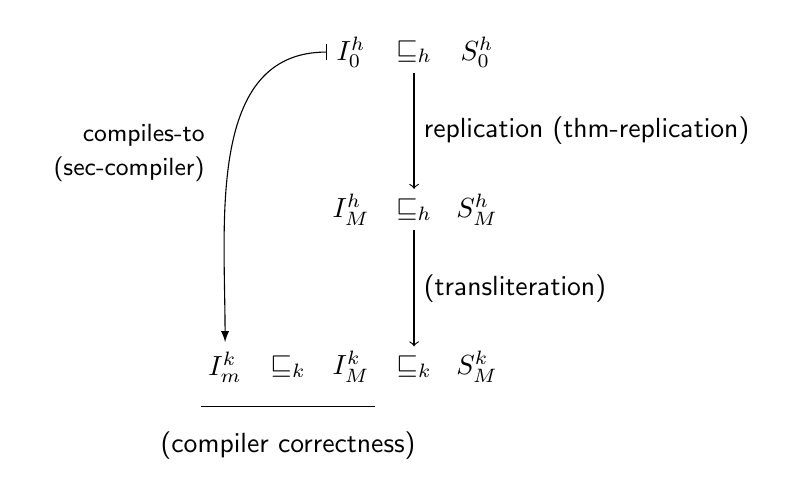
\begin{tikzpicture}
    \node (ih0) at (0, 0) {$I^{h}_{0}$};
    \node (rh0) at (0.8, 0) {$\sqsubseteq_{h}$};
    \node (sh0) at (1.6, 0) {$S^{h}_{0}$};

    \node (ihM) at (0, -2.0) {$I^{h}_{M}$};
    \node (rhM) at (0.8, -2.0) {$\sqsubseteq_{h}$};
    \node (shM) at (1.6, -2.0) {$S^{h}_{M}$};

    \node (ikm) at (-1.6, -4.0) {$I^{k}_{m}$};
    \node (rkm) at (-0.8, -4.0) {$\sqsubseteq_{k}$};
    \node (ikM) at (0, -4.0) {$I^{k}_{M}$};
    \node (rkM) at (0.8, -4.0) {$\sqsubseteq_{k}$};
    \node (skM) at (1.6, -4.0) {$S^{k}_{M}$};

    \draw (-1.9, -4.5) to (0.3, -4.5);
    \node (compCorrect) at (-0.8, -5.0) {\sf{(compiler correctness)}};

    \draw[|-{latex}] (ih0) to[out=180,in=90] node[left] {
      \small\sf\begin{tabular}{r}
      compiles-to\\
      (\autoref{sec-compiler})
      \end{tabular}} (ikm);
    \draw[->] (rh0) to node[right] {\sf{replication (\autoref{thm-replication})}} (rhM);
    \draw[->] (rhM) to node[right] {\sf{(transliteration)}} (rkM);
  \end{tikzpicture}
  \caption{A single-line protocol, a multiline spec, and multiline implementations}
  \label{fig-multiline-spec}
\end{figure}

\autoref{fig-multiline-spec} elaborates more on the role of the multiline specification.
For a given \hemiola{} single-line protocol ($I^{h}_{0}$), we can lift the refinement using the replication theorem to obtain a refinement for the multiline protocol ($I^{h}_{M}$).
Since both \hemiola{} and Kami are rule-based description languages, we expect it is straightforward to have an ideal multiline protocol in Kami ($I^{k}_{M}$) in the sense of simple transliteration, while preserving the refinement.
After all, the correctness of the protocol compiler must be the refinement from a target Kami implementation ($I^{k}_{m}$) to the multiline protocol.
In proving this refinement, \autoref{thm-kami-modular-subst} will be required, since every pipelined cache module in $I^{k}_{m}$ should be substituted to a naive module in $I^{k}_{M}$, transliterated from $I^{h}_{M}$.

As presented in \autoref{fig-multiline-spec}, proving the compiler correctness is a part of the correctness proof of a cache-coherent memory subsystem implementation at the lower level.
While this thesis only focuses on proving cache-coherence protocols described in the high level, we believe that proving the low-level implementation in this manner is another great milestone.

\section{Synthesis of a \hemiola{} Protocol}
\label{sec-synthesis}

\chapter{Related Work II: Verification of Cache-Coherence Protocols}
